% ------------------------------------------------------------------------------
% TYPO3 Version 10.4 - What's New (German Version)
%
% @license	Creative Commons BY-NC-SA 3.0
% @link		https://typo3.org/help/documentation/whats-new/
% @language	German
% ------------------------------------------------------------------------------

\section{Einführung}
\begin{frame}[fragile]
	\frametitle{Einführung}

	\begin{center}\huge{Einführung}\end{center}
	\begin{center}\huge{\color{typo3darkgrey}\textbf{Fakten}}\end{center}

\end{frame}

% ------------------------------------------------------------------------------
% TYPO3 Version 10.4 - The Facts

\begin{frame}[fragile]
	\frametitle{Einführung}
	\framesubtitle{TYPO3 Version 10.4 - Fakten}

	\begin{itemize}
		\item Veröffentlichungsdatum: 21. April 2020
		\item Releasetyp: LTS (Langfristiger Support)
	\end{itemize}

	\begin{figure}
		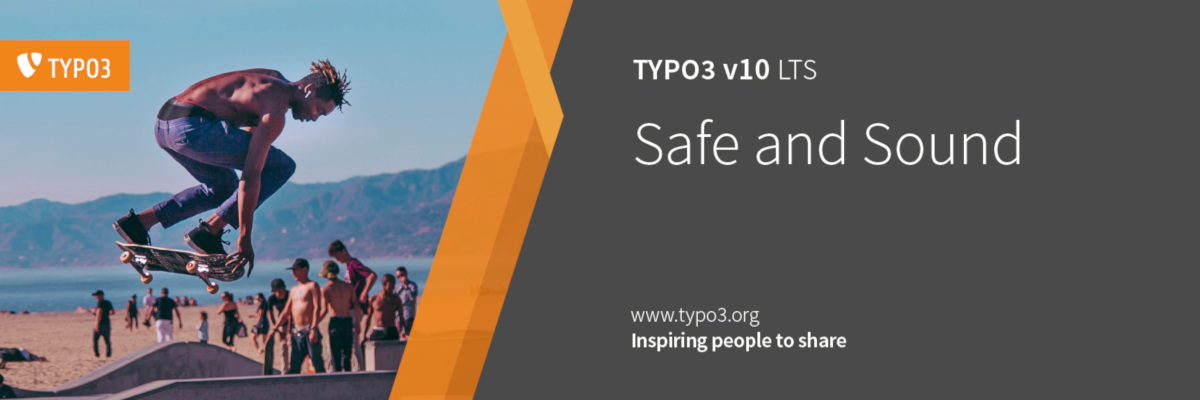
\includegraphics[width=0.95\linewidth]{Introduction/typo3-v10-4-banner.jpg}
	\end{figure}

\end{frame}

% ------------------------------------------------------------------------------
% TYPO3 Version 10.4 - Executive Summary

\begin{frame}[fragile]
	\frametitle{Einführung}
	\framesubtitle{Zusammenfassung}

	\small
		TYPO3 v10.4 (auch TYPO3 v10 LTS genannt, was darauf hindeutet, dass es sich um eine Langzeit-Support-Version 		     handelt)ist unser neues Vorbild und ohne Zweifel eines der fortschrittlichsten PHP-basierten Open-Source-Content- Management-Systeme auf dem Markt.

		\vspace{0.2cm}

		Nachdem wir seit Juli 2019 fünf Sprint-Releases veröffentlicht haben, können wir mit Stolz behaupten,
		dass wir TYPO3 mit den modernsten PHP-Libraries ausgestattet haben und dass wir einige fantastische neue
		Enterprise-Funktionen eingefügt haben.

		\vspace{0.2cm}

		Bitte beachten Sie, dass dieses Dokument nur die Änderungen zwischen TYPO3 v10.3 und v10.4 zusammenfasst.

		\vspace{0.2cm}

		Die "What's New Slides" aller TYPO3 v10.x-Versionen sind verfügbar unter
		\href{https://typo3.org/help/documentation/whats-new/}{typo3.org}.

	\normalsize

\end{frame}

% ------------------------------------------------------------------------------
% System Requirements

\begin{frame}[fragile]
	\frametitle{Einführung}
	\framesubtitle{Systemvoraussetzungen}

	\begin{itemize}
		\item PHP Version 7.2, 7.3 oder 7.4
		\item PHP Einstellungen:

			\begin{itemize}
				\item \texttt{memory\_limit} >= 256M
				\item \texttt{max\_execution\_time} >= 240s
				\item \texttt{max\_input\_vars} >= 1500
				\item Die Komplilierungsoption \texttt{-}\texttt{-disable-ipv6} darf \underline{nicht} benutzt werden
			\end{itemize}

		\item Die meisten von \textbf{Doctrine DBAL} unterstützten Datenbankserver funktionieren auch mit TYPO3.
			Getested DB-Engines sind zum Beispiel:
	\end{itemize}

	\begin{figure}
		
\includegraphics[width=0.80\linewidth]{Introduction/logo-databases.png}
	\end{figure}

\end{frame}

% ------------------------------------------------------------------------------
% Development, Release, and Maintenance Timeline

\begin{frame}[fragile]
	\frametitle{Einführung}
	\framesubtitle{Zeitplan für Entwicklung, Veröffentlichung und Instandhaltung}

	\textbf{TYPO3 v10}

	\begin{figure}
		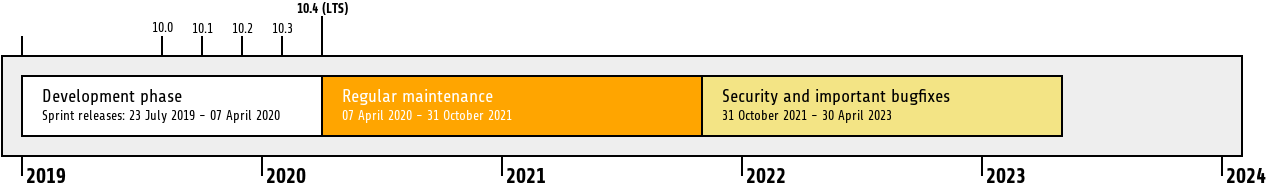
\includegraphics[width=1\linewidth]{Introduction/typo3-v10-lifecycle.png}
	\end{figure}

	\textbf{Erweiterter Support}\newline
	\smaller
		Die \href{https://typo3.com}{TYPO3 GmbH} bietet weitere Supportmöglichkeiten
		für TYPO3 v10 LTS auch nach 30. April 2023 für bis zu zwei weitere Jahre.
	\normalsize

\end{frame}

% ------------------------------------------------------------------------------
% TYPO3 v10 Roadmap

\begin{frame}[fragile]
	\frametitle{Einführung}
	\framesubtitle{TYPO3 v10 Roadmap}

	Veröffentlichungsdaten und ihr Hauptfokus:

	\begin{itemize}

		\item v10.0 \tabto{1.1cm}23/July/2019\tabto{3.4cm}Pave the way for exciting new concepts and APIs
		\item v10.1 \tabto{1.1cm}01/Oct/2019\tabto{3.4cm}Routing Improvements and Site Handling v2
		\item v10.2 \tabto{1.1cm}03/Dec/2019\tabto{3.4cm}Fluid/Rendering Engine Improvements
		\item v10.3 \tabto{1.1cm}25/Feb/2020\tabto{3.4cm}Feature Freeze
		\item
			\begingroup
				\color{typo3orange}
				v10.4 \tabto{1.1cm}21/Apr/2020\tabto{3.4cm}LTS Release (long-term support)
			\endgroup

	\end{itemize}

	\vspace{0.6cm}
	\smaller
		\url{https://typo3.org/article/typo3-v10-roadmap}\newline
		\url{https://typo3.org/article/typo3-v10-lts-safe-and-sound}
	\normalsize

\end{frame}

% ------------------------------------------------------------------------------
% Installation

\begin{frame}[fragile]
	\frametitle{Einführung}
	\framesubtitle{Installation}

	\begin{itemize}
		\item Offizielles \textit{klassisches} Installationverfahren unter Linux/Mac OS X\newline
			(DocumentRoot zum Beispiel \texttt{/var/www/site/htdocs}):
\begin{lstlisting}
$ cd /var/www/site
$ wget --content-disposition get.typo3.org/10.4
$ tar xzf typo3_src-10.4.0.tar.gz
$ cd htdocs
$ ln -s ../typo3_src-10.4.0 typo3_src
$ ln -s typo3_src/index.php
$ ln -s typo3_src/typo3
$ touch FIRST_INSTALL
\end{lstlisting}

		\item Symbolische Links unter Microsoft Windows:

			\begin{itemize}
				\item Unter Windows XP/2000 kann \texttt{junction} benutzt werden 
				\item Unter Windows Vista und Windows 7 oder höher kann \texttt{mklink} benutzt werden
			\end{itemize}

	\end{itemize}
\end{frame}

% ------------------------------------------------------------------------------
% Installation using composer

\begin{frame}[fragile]
	\frametitle{Installation und Upgrade}
	\framesubtitle{Installation mit \texttt{composer}}

	\begin{itemize}
		\item Installation mit \textit{composer} unter Linux, Mac OS X und Windows 10:
\begin{lstlisting}
$ cd /var/www/site/
$ composer create-project typo3/cms-base-distribution typo3v10 ^10.4
\end{lstlisting}

		\item Alternativ eine benutzerdefinierte \texttt{composer.json} Datei erstellen und ausführen:
\begin{lstlisting}
$ composer install
\end{lstlisting}

			Weitere Details zum Composer für den TYPO3-Kern und für TYPO3-Erweiterungen finden
			Sie unter:

			\small
				\href{https://get.typo3.org/misc/composer/repository}{https://get.typo3.org/misc/composer/repository}
			\normalsize

	\end{itemize}
\end{frame}

% ------------------------------------------------------------------------------
